\documentclass[titlepage]{ltjsbook}
\usepackage[
  paperheight=232truemm, paperwidth=182truemm,
  top=20truemm, bottom=15truemm, inner=15truemm, outer=15truemm
  ]{geometry}

%\documentclass[tombow, paper={182truemm, 232truemm}, titlepage]{ltjsbook}
\usepackage{amsmath}
\usepackage{amsfonts}
\usepackage{amssymb}
\usepackage{mathtools}
\usepackage{mathrsfs}

\usepackage{textgreek}
\usepackage[luatex]{graphicx} 
%\usepackage[draft]{graphicx}
\usepackage{sidecap}
\usepackage[most]{tcolorbox}

\usepackage[svgnames]{xcolor}
\usepackage{sty/julia-syntax-highlighting} % 
\usepackage{sty/indexing} % 

\usepackage[export]{sty/adjustbox} % added

\usepackage{fancyhdr}
\pagestyle{fancy}
\fancyfoot{}
\fancyhead[RO, LE]{\thepage}
\fancyhead[LO]{\nouppercase{\leftmark}}
\fancyhead[RE]{\nouppercase{\rightmark}}

%\renewcommand{\chaptermark}[1]{\markboth{#1}{} }
\renewcommand{\chaptermark}[1]{\markboth{第\ \thechapter\ 章. ~#1}{}}
% \renewcommand{\chaptermark}[1]{\markboth{\MakeUppercase{第\chaptername \thechapter 章.\ #1}}{}}
% \renewcommand{\headrulewidth}{0pt}

\usepackage{hyperref}

% https://ja.overleaf.com/learn/latex/Bibliography_management_with_bibtex
\usepackage[
    backend=biber,
    bibencoding=utf8,
    style=authoryear-comp, 
    url=false,
    isbn=true,
    doi=true,
    natbib=true, 
    alldates=year,
    maxcitenames=2,
    uniquelist=false, 
    sorting=nty,
    sortcites=true,
    giveninits=true,
    terseinits=false,
    refsegment=chapter
]{biblatex}

\addbibresource{../references/03_credit-assignment-problem.bib}

\DeclareNameAlias{author}{last-first}
\AtEveryBibitem{\clearlist{language}}
\renewbibmacro{in:}{}

% https://stackoverflow.com/questions/69682457/extended-links-in-citations
% \makeatletter
% \renewbibmacro*{cite}{%
%   \printtext[bibhyperref]{\iffieldundef{shorthand}
%     {\ifthenelse{\ifnameundef{labelname}\OR\iffieldundef{labelyear}}
%        {\usebibmacro{cite:label}%
%         \setunit{\printdelim{nonameyeardelim}}}
%        {\printnames{labelname}%
%         \setunit{\printdelim{nameyeardelim}}}%
%      \usebibmacro{cite:labeldate+extradate}}
%     {\usebibmacro{cite:shorthand}}}}
% \makeatother

\newcommand{\jl}{\lstinline[language=julia]}

\title{\Huge \textbf{Juliaで作って学ぶ計算論的神経科学}}
\author{\huge 山本 拓都}
\date{\huge \today} 

\begin{document}
%\maketitle
\setcounter{tocdepth}{2}
\tableofcontents
\clearpage
\chapter{貢献度分配問題とニューラルネットワーク}
\section{再帰型ニューラルネットワークと経時的貢献度分配問題}
本節では再帰型ニューラルネットワーク(recurrent neural networks; RNN),すなわち再帰的結合を持った発火率モデルの学習則について取り扱う.前節までで扱った前方向結合のみのニューラルネットワークでは通常,入力と出力の間の遅延は考慮せず,即時的に学習することを想定する。しかしRNNや運動制御,強化学習などの動的な系では,シナプス結合,神経活動や行動の変化が,誤差や報酬という形で観測されるまでに時間的な遅れを伴う場合がある。このような状況において,「ある時点のシナプス結合,神経活動,行動等の変化が,後になって得られる誤差や報酬にどれだけ寄与したか」を明らかにし,各変化に対して貢献度を適切に割り当てる問題を経時的貢献度分配問題(temporal credit assignment problem; TCAP)と呼ぶ。

勾配法に基づいて経時的貢献度分配をする代表的な手法として,実時間再帰学習 (real-time recurrent learning; RTRL) と経時的誤差逆伝播法  (backpropagation through time; BPTT) の2種類がある.本節ではまず,RTRLとBPTTを勾配和の方向に基づいた統合的な視点から説明し,なぜ勾配法から2種類の学習則が得られるのかについて説明する.次に,RTRLとBPTTを用いてパラメータの勾配を具体的に計算する.最後に,RTRLとBPTTを踏まえたうえで,生理学的妥当性の高い学習則について説明を行う.

\section{勾配法に基づく経時的貢献度分配}
\subsection{RNNの構造と損失関数}
まず,本節で扱うRNNの定義を行う.時刻 $t\ (1\leq t \leq T)$\footnote{隠れ状態 $\mathbf{h}_t$ についてのみ $t=0$ を定義する.} における入力を $\mathbf{x}_t \in \mathbb{R}^{n}$,隠れ状態を $\mathbf{h}_t \in \mathbb{R}^{d}$,出力を $\mathbf{y}_t \in \mathbb{R}^{m}$ とすると,隠れ状態と出力は
\begin{align}
\mathbf{u}_t &= \mathbf{W}_{\mathrm{rec}}\mathbf{h}_{t-1} + \mathbf{W}_{\mathrm{in}}\mathbf{x}_t + \mathbf{b}_\mathrm{rec}\\
\mathbf{h}_t &= \left(1-\alpha\right)\mathbf{h}_{t-1} + \alpha f(\mathbf{u}_t)\\
\mathbf{v}_t &= \mathbf{W}_{\mathrm{out}}\mathbf{h}_t+ \mathbf{b}_\mathrm{out}\\
\mathbf{y}_t &= g(\mathbf{v}_t)
\end{align}  
で与えられる。ただし,$\mathbf{W}_{\mathrm{in}} \in \mathbb{R}^{d\times n}, \mathbf{W}_{\mathrm{rec}} \in \mathbb{R}^{d\times d}, \mathbf{W}_{\mathrm{out}} \in \mathbb{R}^{m\times d}$ はシナプス結合重み,$\mathbf{b}_\mathrm{rec} \in \mathbb{R}^{d}, \mathbf{b}_\mathrm{out} \in \mathbb{R}^{m}$ は定常項である.$f(\cdot), g(\cdot)$ は活性化関数であり,入力ベクトルの要素ごとに作用する.$\mathbf{u}_t, \mathbf{v}_t$ は膜電位に対応し,勾配を書き下す際に使用する.$\alpha:=\frac{1}{\tau}$ は状態の更新率(時定数 $\tau$ の逆数)であり \footnote{$\alpha < 1$であるRNNは,重み共有をした残差結合 (residual/skip connection) のある順伝播モデル (ResNetなど) に展開することが可能である \citep{liao2016bridging}.},
$\alpha = 1$ の場合はElmanネットワーク \citep{elman1990finding} と同一である.なお,状態の初期値を $\mathbf{h}_{0}=\mathbf{0}$ とする.時刻 $t$ での教師信号を $\mathbf{y}_t^*$ とすると,損失 $\mathcal{L}$ は各時刻における損失 $\mathcal{L}_t$ の和を取り,
\begin{equation}
\mathcal{L} = \sum_{t=1}^T \mathcal{L}_t\left(\mathbf{y}_t,\mathbf{y}_t^*\right)
\end{equation}  
として与えられる.

\subsection{未来方向・過去方向の勾配和}
このRNNを学習させる際の目標は,損失 $\mathcal{L}$ を最小化するようにパラメータ $\theta$ を最適化することである.ここでは,$\theta \in\{\mathbf{W}_{\mathrm{in}},\mathbf{W}_{\mathrm{rec}},\mathbf{W}_{\mathrm{out}},\mathbf{b}_\mathrm{rec}, \mathbf{b}_\mathrm{out}\}$ である.

勾配法の観点では,損失のパラメータに対する勾配 $\dfrac{\partial \mathcal{L}}{\partial \theta}$ が求まれば最適化が可能である.損失は $\mathcal{L} = \sum_t \mathcal{L}_t$ と時間方向に分解できるので,勾配は
\begin{align}
\frac{\partial \mathcal{L}}{\partial \theta}&=\sum_{t=1}^T\frac{\partial \mathcal{L}_t}{\partial \theta}=\sum_{t=1}^T\sum_{s=1}^T\frac{\partial \mathcal{L}_t}{\partial \theta_s}\underbrace{\frac{\partial \theta_s}{\partial \theta}}_{= \mathbf{I}}=\sum_{t=1}^T\sum_{s=1}^t\frac{\partial \mathcal{L}_t}{\partial \theta_s}
\end{align}
と時間方向に分解できる.ここで,$s, t$ はいずれも時刻を表し,$1 \leq s, t \leq T$ である.また,便宜的に「時刻 $s$ に用いられたパラメータ $\theta$」を $\theta_s$ と表記した。従って,$\dfrac{\partial \mathcal{L}_t}{\partial \theta_s}$ は「時刻 $t$ における損失 $\mathcal{L}_t$ の時刻 $s$ に用いられたパラメータ $\theta_s$ に対する勾配」を意味する。また,オンライン学習でパラメータを毎時刻更新する場合であっても,勾配計算においては $\theta_s$ の微小変化 $\delta \theta_s$ はそのまま現在の $\theta$ の微小変化  $\delta \theta$ に等しいと見なせるため,$\dfrac{\partial \theta_s}{\partial \theta} = \mathbf{I}$ が成立する。さらに現在のパラメータの状態は過去の損失に影響を与えないため,$s>t$ では $\dfrac{\partial \mathcal{L}_t}{\partial \theta_s}=\mathbf{0}$ となり,上式では $s\leq t$ の範囲の勾配のみが残っている.

ここで,なぜBPTTとRTRLの2種類の学習法が存在するのかを考えると、$\displaystyle \sum_{t}\sum_{s\leq t}\dfrac{\partial \mathcal{L}_t}{\partial \theta_s}$ という二重和において、どちらの変数に対して先に和を取るかに2通りの方法があるためである。すなわち、現在時刻を $t$ または $s$ のいずれかを基準にとるかによって、内側の和を未来方向 (future-facing) または過去方向 (past-facing)に進めることができ、これに応じて勾配の和の取り方も区別される \citep{marschall2020unified}:
\begin{align}
\frac{\partial \mathcal{L}}{\partial \theta}=
\begin{dcases}
\sum_{s=1}^T\frac{\partial \mathcal{L}}{\partial \theta_s}=\sum_{s=1}^T\sum_{t=s}^T\frac{\partial \mathcal{L}_t}{\partial \theta_s}\quad(\text{未来方向勾配和; e.g., BPTT})\\
\sum_{t=1}^T\frac{\partial \mathcal{L}_t}{\partial \theta}=\sum_{t=1}^T\sum_{s=1}^t\frac{\partial \mathcal{L}_t}{\partial \theta_s}\quad(\text{過去方向勾配和; e.g., RTRL})
\end{dcases}
\end{align}
未来方向勾配和では、「現在時刻 $s$ におけるパラメータ $\theta_s$ が、未来のすべての損失 $\mathcal{L}_t\ (t \geq s)$ に与える影響」を合算する。したがって、この形式では、「現在のパラメータの微小な変化が将来の損失にどれだけ影響を及ぼすか」を評価することになる。未来方向勾配和を利用する手法の代表例がBPTTである.一方、過去方向勾配和では、「現在時刻 $t$ における損失 $\mathcal{L}_t$ に対して、過去のすべてのパラメータ $\theta_s\ (s \leq t)$ が及ぼした影響」を合算する。すなわち、この形式では、「現在の損失が過去のパラメータの微小な変化にどれだけ応答するか」を評価することになる。過去方向勾配和を利用する手法の代表例がRTRLである.これらの勾配和についての概念図が図 \ref{fig:bptt_rtrl} である.

\begin{figure}[htbp]
\begin{center}
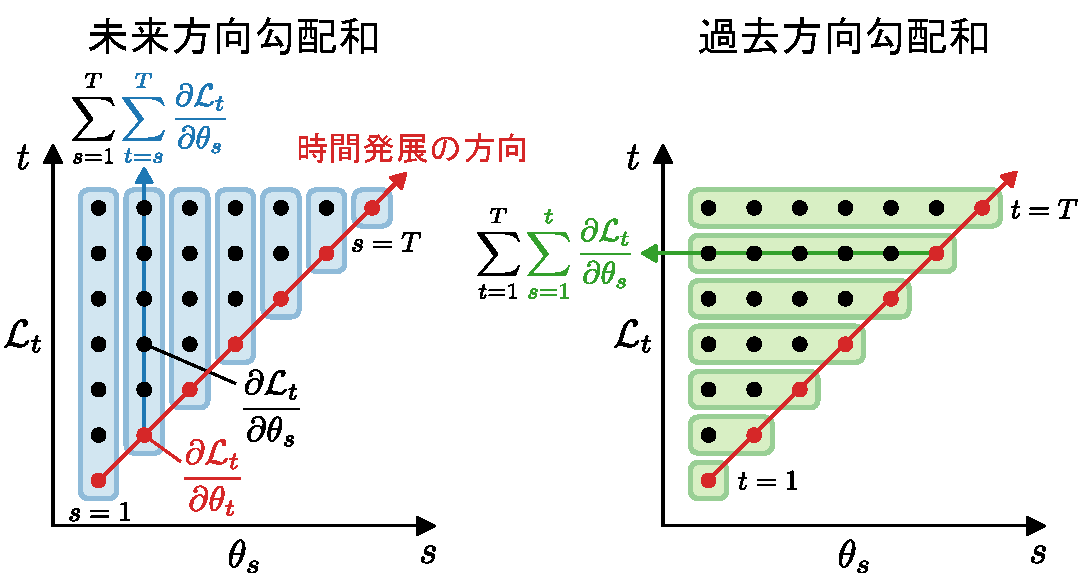
\includegraphics[width=0.8\textwidth]{./figures/bptt_rtrl.pdf}
\caption{未来方向勾配和(左)と過去方向勾配和(右)の模式図.縦軸の $t$ は損失関数 $\mathcal{L}$ の時刻を表し,横軸の $s$ はパラメータ $\theta$ の時刻を表す.モデルの時間発展は赤点に従って行われる.各点は $\dfrac{\partial \mathcal{L}_t}{\partial \theta_s}$ を意味する.対角線においては $s=t$ であるため,赤点は $\dfrac{\partial \mathcal{L}_t}{\partial \theta_t}$ を意味する.囲まれた点の集まりは,時刻 $t$ において,どの勾配を考慮するか,ということを意味する.}
\label{fig:bptt_rtrl}
\end{center}
\end{figure}

勾配和をいずれの方向で取る場合であっても、二重和をそのまま計算すれば、計算量は $\mathcal{O}(T^2)$ となり、非効率である。このため、動的計画法 (dynamic programming; DP) を用いて、計算量を $\mathcal{O}(T)$ に削減するのが一般的である。ここで,動的計画法とは、問題を部分問題に分割し、それらの部分問題の解を再利用することで、全体の計算量を削減するアルゴリズム設計手法である。誤差逆伝播法(backpropagation)も動的計画法の一種に位置づけられ、また、運動制御や強化学習など、さまざまな分野で動的計画法は頻繁に用いられている。

なお,BPTTとRTRLをある程度ご存じの読者であれば,「BPTTは過去方向でRTRLは未来方向ではないのか」という疑問が浮かぶであろう.ここで「勾配和の評価において時間を進める方向」と「動的計画法において計算を進める方向」は逆になることに注意していただきたい.例えば、未来向き勾配和のように,将来に発生する損失や報酬を考慮して損失関数を評価する場合、動的計画法を適用すると、計算は未来から過去へと逆向きに進める必要がある。このように、将来の結果をもとに現在の値を推定する構図は、強化学習のTD学習における状態価値の推定にも見られる。すなわち、状態価値を将来の累積報酬の期待値として定義した上で、その推定は未来から過去へと逆向きに進められる\footnote{TD学習を含め,強化学習は第11章で詳解する.}。

以上を踏まえ,勾配和を動的計画法を用いて計算しよう.動的計画法を適用するためには、まず勾配を適切に展開し,現在の勾配を、ひとつ前(または後)の時刻における勾配との関係で再帰的に表現する必要がある。このとき留意すべき基本原則は、「現在の状態やパラメータは、過去の損失、状態、パラメータに影響を及ぼさない」という事実である。すなわち、現在の変数に対する過去の変数の勾配は常に0となる.これは例えば $\dfrac{\partial \mathbf{h}_{t-1}}{\partial \mathbf{h}_t}=\mathbf{0}$ が成り立つ。一方で、未来の変数は現在の変数に依存するため、現在の変数が未来の損失に及ぼす影響は意味を持つ。したがって、勾配を展開する際には、未来の損失に向かう方向で連鎖律を適用していくことになる。

まず,未来方向勾配和の場合を考える.即時的なパラメータに対する損失の勾配は,
\begin{align}
\frac{\partial \mathcal{L}}{\partial \theta_t}&=\frac{\partial \mathcal{L}}{\partial \mathbf{h}_t}\frac{\partial \mathbf{h}_t}{\partial \theta_t}=\left(\sum_{s \geq t} \frac{\partial \mathcal{L}_s}{\partial \mathbf{h}_t} \right)\frac{\partial \mathbf{h}_t}{\partial \theta_t}\\
&=\left(\frac{\partial \mathcal{L}_t}{\partial \mathbf{h}_t} + \sum_{s \geq t+1} \frac{\partial \mathcal{L}_s}{\partial \mathbf{h}_t} \right)\frac{\partial \mathbf{h}_t}{\partial \theta_t}\\
&=\left(\frac{\partial \mathcal{L}_t}{\partial \mathbf{h}_t} + \sum_{s \geq t+1} \frac{\partial \mathcal{L}_s}{\partial \mathbf{h}_{t+1}}\frac{\partial \mathbf{h}_{t+1}}{\partial \mathbf{h}_t} \right)\frac{\partial \mathbf{h}_t}{\partial \theta_t}\\
&=\left(\frac{\partial \mathcal{L}_t}{\partial \mathbf{h}_t} + \frac{\partial \mathcal{L}}{\partial \mathbf{h}_{t+1}}\frac{\partial \mathbf{h}_{t+1}}{\partial \mathbf{h}_t} \right)\frac{\partial \mathbf{h}_t}{\partial \theta_t}
\end{align}
となる.ここで貢献度分配ベクトル (credit assignment vector) を $\boldsymbol{\delta}_t := \dfrac{\partial \mathcal{L}}{\partial \mathbf{h}_t} \in \mathbb{R}^{1\times d}$,即時的貢献度分配ベクトルを $\tilde{\boldsymbol{\delta}}_t := \dfrac{\partial \mathcal{L}_t}{\partial \mathbf{h}_t} \in \mathbb{R}^{1\times d}$,状態遷移のヤコビ行列を $\mathbf{J}_t := \dfrac{\partial \mathbf{h}_{t}}{\partial \mathbf{h}_{t-1}} \in \mathbb{R}^{d\times d}$ とすると,$\boldsymbol{\delta}_t$ は次のように未来から過去に向かう再帰的な関係式で表せる:
\begin{equation}
\boldsymbol{\delta}_t=\tilde{\boldsymbol{\delta}}_t + \boldsymbol{\delta}_{t+1}\mathbf{J}_{t+1}
\end{equation}
ただし,境界条件として $\boldsymbol{\delta}_{T+1}=\mathbf{0}$ とする。この式を用いて,$\boldsymbol{\delta}_t$ を逐次的に求め,$\dfrac{\partial \mathbf{h}_t}{\partial \theta_t}$ を即時的に計算して $\boldsymbol{\delta}_t$ に乗じれば,$\dfrac{\partial \mathcal{L}}{\partial \theta_t}$ が求まる.

次に過去方向勾配和の場合を考える.パラメータに対する即時的な損失の勾配は
\begin{align}
\frac{\partial \mathcal{L}_t}{\partial \theta}&=\frac{\partial \mathcal{L}_t}{\partial \mathbf{h}_t}\frac{\partial \mathbf{h}_t}{\partial \theta}=\frac{\partial \mathcal{L}_t}{\partial \mathbf{h}_t}\left(\sum_{s\leq t} \frac{\partial \mathbf{h}_t}{\partial \theta_s}\right)\\
&=\frac{\partial \mathcal{L}_t}{\partial \mathbf{h}_t}\left(\frac{\partial \mathbf{h}_t}{\partial \theta_t} + \sum_{s\leq t-1} \frac{\partial \mathbf{h}_t}{\partial \theta_s}\right)\\
&=\frac{\partial \mathcal{L}_t}{\partial \mathbf{h}_t}\left(\frac{\partial \mathbf{h}_t}{\partial \theta_t} + \sum_{s\leq t-1} \frac{\partial \mathbf{h}_t}{\partial \mathbf{h}_{t-1}}\frac{\partial \mathbf{h}_{t-1}}{\partial \theta_s}\right)\\
&=\frac{\partial \mathcal{L}_t}{\partial \mathbf{h}_t}\left(\frac{\partial \mathbf{h}_t}{\partial \theta_t} + \frac{\partial \mathbf{h}_t}{\partial \mathbf{h}_{t-1}}\frac{\partial \mathbf{h}_{t-1}}{\partial \theta}\right)
\end{align}
となる.ここで感度行列 (sensitivity matrix, influence matrix) を $\mathbf{P}_t:=\dfrac{\partial \mathbf{h}_t}{\partial \theta}\in \mathbb{R}^{d \times |\theta|}$,即時的感度行列を $\tilde{\mathbf{P}}_t:=\dfrac{\partial \mathbf{h}_t}{\partial \theta_t}\in \mathbb{R}^{d \times |\theta|}$ とする.ただし,$|\theta|$ はパラメータの次元数を意味する.この場合,$\mathbf{P}_t$ は次のように過去から未来に向かう再帰的な関係式で表せる:
\begin{equation}
\mathbf{P}_t=\tilde{\mathbf{P}}_t + \mathbf{J}_{t}\mathbf{P}_{t-1}
\end{equation}
ただし,境界条件として $\mathbf{P}_{0}=\mathbf{0}$ とする。この式を用いて,$\mathbf{P}_t$ を逐次的に求め,$\dfrac{\partial \mathcal{L}_t}{\partial \mathbf{h}_t}$ を即時的に計算して $\mathbf{P}_t$ に乗じれば,$\dfrac{\partial \mathcal{L}_t}{\partial \theta}$ が求まる.

連鎖律に基づき理論的な勾配導出を行ったが、数値計算においては、誤差逆伝播法における処理と同様に、自動微分(automatic differentiation, AD)の枠組みを適用して勾配を効率的に計算することができる。自動微分では、微分の累積過程に応じて2つのモードがあり,それぞれが勾配和の2つの方向と対応する。すなわち、未来方向に対する勾配和の計算は逆方向累積(reverse accumulation)または逆モード(reverse-mode)自動微分によって、過去方向に対する勾配和の計算は順方向累積(forward accumulation)または順モード(forward-mode)自動微分によって、それぞれ実行される.

本節の最後に、パラメータに対する損失勾配の展開を整理する。すなわち、未来方向(BPTTに相当)および過去方向(RTRLに相当)での勾配和は、それぞれ次のように表される。
\begin{tcolorbox}[ams equation*]
\begin{alignedat}{3}
\text{未来方向勾配和}:\quad&\frac{\partial \mathcal{L}}{\partial \theta} =
&&\sum_{t=1}^T \frac{\partial \mathcal{L}}{\partial \theta_t}
= \sum_{t=1}^T \frac{\partial \mathcal{L}}{\partial \mathbf{h}_t} \frac{\partial \mathbf{h}_t}{\partial \theta_t}
&&= \sum_{t=1}^T \left( \frac{\partial \mathcal{L}_t}{\partial \mathbf{h}_t} + \frac{\partial \mathcal{L}}{\partial \mathbf{h}_{t+1}} \frac{\partial \mathbf{h}_{t+1}}{\partial \mathbf{h}_t} \right) \frac{\partial \mathbf{h}_t}{\partial \theta_t}\\
\text{過去方向勾配和}:\quad&\frac{\partial \mathcal{L}}{\partial \theta} =
&&\sum_{t=1}^T \frac{\partial \mathcal{L}_t}{\partial \theta}
= \sum_{t=1}^T \frac{\partial \mathcal{L}_t}{\partial \mathbf{h}_t} \frac{\partial \mathbf{h}_t}{\partial \theta}
&&= \sum_{t=1}^T \frac{\partial \mathcal{L}_t}{\partial \mathbf{h}_t} \left( \frac{\partial \mathbf{h}_t}{\partial \theta_t} + \frac{\partial \mathbf{h}_t}{\partial \mathbf{h}_{t-1}} \frac{\partial \mathbf{h}_{t-1}}{\partial \theta} \right)
&&
\end{alignedat}
\end{tcolorbox}
次節 (BPTT) および次々節 (RTRL) では、ここで導出した関係式に基づいて、各パラメータの勾配を具体的に計算する。
\printbibliography[segment=\therefsegment,heading=subbibliography,title={参考文献}]
\addcontentsline{toc}{section}{参考文献}
\end{document}